%% storify source: the close-out report of the "peeling the onion" run.
%% Edit THIS file. Run `python3 build_story.py` to write report.tex, then
%% `latexmk -pdf report.tex`. Never edit report.tex by hand: the build overwrites it.
%%
%% numbers   every measured number is a macro that the build defines in the data slot.
%% typed     \lit{} constants (design constants, names that hold digits, dates):
%%           3 seeds, 80,000 windows, 16 / 256 / 8 / 32 regions, 25 bp, 25.6 kb, 1,024 bins,
%%           36 tracks, 36 / 50 bp crops, 11 columns, 2^24 and 2^23 reads, U(0.2, 0.8),
%%           0.25 bin mask, 10^-3 learning rate, 0 and 1 (metric scale ends),
%%           0.5 / 0.25 / 0.25 composite weights, version 3, 95% (interval level),
%%           1.5 (seed-range ratio), 5 Mb (shift control), 4 (loss weight), 1/1/1 weights,
%%           10% (lambda tolerance), 500 bp tiles, -log10 p >= 2, seed 0, 21 arm folders,
%%           24 hours, AlphaGenome 2, condition numbers 1 to 6, criterion numbers 1 to 4,
%%           H3K36me3, eic_v1, eic_v1_2, dates 2026-11-10 to 2026-11-20, 1 bp,
%%           the estimability rule (5 pairs from 3 cells), decision numbers 1 to 9.
%% VERSION 2 (2026-11-18): the replicate ladder, the second-experiment layers, the side
%%           deliverables, the rescoring status and the PI decisions of 2026-11-17.
%%
%% RESCORING. One paragraph (between the RESCORING-PARAGRAPH marks) and one table (between
%% the RESCORING-TABLE marks) wait for the 256-region rescoring of the 7 decisive arms.
%% Copy the arm summary to results/rescoring_p256/arm_summary_p256_sv.tsv, rebuild (the
%% table fills itself), then rewrite the paragraph with build macros.
\documentclass[pdflatex,sn-mathphys-num]{sn-jnl}

% crux-sources: __SOURCES__

\usepackage{graphicx}
\usepackage{amsmath}
\usepackage{booktabs}
\usepackage{xcolor}
\usepackage{tikz}
\usetikzlibrary{positioning,arrows.meta,calc,fit}
\usepackage{pgfplots}
\pgfplotsset{compat=1.18}
\usepgfplotslibrary{groupplots}
\usepackage{pgfplotstable}
\usepackage{url}
\geometry{textwidth=15.5cm,textheight=23cm,centering}

% A design constant or a name with digits, typed in prose. It renders its argument.
\newcommand{\lit}[1]{#1}
% The PI's mark for prose drafted by an agent. Identity by default.
% To colour it: \renewcommand{\cl}[1]{{\color{teal}#1}}
\newcommand{\cl}[1]{#1}
% Column headers that span two or three columns.
\newcommand{\mcthree}[1]{\multicolumn{3}{c}{#1}}
\newcommand{\mctwo}[1]{\multicolumn{2}{c}{#1}}

\definecolor{mAE}{HTML}{3F7D7A}
\definecolor{mAT}{HTML}{C08A2E}
\definecolor{mUN}{HTML}{B5462E}
\definecolor{mgray}{HTML}{6B6B6B}

% __DATA__

\raggedbottom
\renewcommand{\topfraction}{0.9}\renewcommand{\bottomfraction}{0.8}\renewcommand{\textfraction}{0.07}\renewcommand{\floatpagefraction}{0.75}
\setcounter{topnumber}{3}\setcounter{bottomnumber}{2}\setcounter{totalnumber}{5}

\begin{document}

\title[Peeling the onion: close-out]{Peeling the onion: augmented EIC data, a defined objective and evaluation, and a provisional miniCANDI design}

\author{\fnm{Mehdi} \sur{Foroozandeh}}
\affil{\orgname{Libbrecht lab, Simon Fraser University. Close-out report, private draft of \lit{2026-11-18}}}

\abstract{\cl{We report the close-out of a run whose aim was to separate the sources of variance in epigenomic count data and to settle a small model, miniCANDI, before scaling. We rebuilt the ENCODE Imputation Challenge data from reads with designed processing views, defined a Negative Binomial training objective, and scored three architectures and \nArmRows{} single-switch ablations with \lit{3} seeds each. No architecture won: the U-Net led on imputation and the two convolutional models led on correction, and on \lit{256} regions the composite of the U-Net was lower than that of the conv autoencoder by \compAeUnAll{}, inside the selection bar of \compAeUnBar{}. Training on the base view only removed most of the correction-only term on all three models (for example \eBoCoAE{}, seed range \eBoCoAEBar{}), but this term was scored on \lit{16} regions, and the pre-written check of \lit{16} against \lit{256} regions failed, so every correction effect stays provisional until a queued rescoring runs.}}

\keywords{epigenome imputation, Negative Binomial, counterfactual views, ablation, ENCODE Imputation Challenge}

\maketitle

\noindent\cl{\textit{Note.} An AI agent (Claude) drafted all text of this report from the files of the run. The PI has not edited it. Every number is read by the build script from a result file and checked against the hash of that file.}

\section{Motivation and background}\label{sec:motivation}

\subsection{The question}

\cl{An epigenomic track is a count of sequencing reads per genomic bin for one assay in one cell type. Its variance has several sources: the biology of the cell, the experiment that produced it (lab, antibody, donor), the processing of the reads (depth, read length, duplicate removal), and the random sampling of reads. The run, called ``peeling the onion'', had three goals for a model: impute a track that was never measured (imputation), turn a track processed one way into the same track processed another way (covariate correction), and give a calibrated predictive distribution (uncertainty). miniCANDI is a model of about one million parameters that predicts a Negative Binomial (NB) distribution, i.e. a count distribution with a mean and a size parameter, per assay and \lit{25}~bp bin. It is the small prototype of the full model.}

\cl{On \lit{2026-11-16} the PI set four success criteria: (\lit{1}) the augmented EIC data with counterfactual views; (\lit{2}) a well-defined training objective; (\lit{3}) a well-defined and tested evaluation; (\lit{4}) a settled and tested miniCANDI design, ready for scaling in the next session. The PI also ordered that this report show whether and where the counterfactual views help. This report answers each criterion with ``delivered'', ``partial'' or ``not delivered'' (Table~\ref{tab:criteria}).}

\begin{table}[!htbp]
\caption{\cl{The four success criteria and their state at the end of the run.}}\label{tab:criteria}
\footnotesize
\begin{tabular}{p{3.3cm}p{1.5cm}p{7.4cm}}
\toprule
criterion & state & evidence and gap \\
\midrule
\lit{1}. Augmented EIC data with counterfactual views & partial & Built: the rebuilt tables with designed views and read halves, the covariate fill (lab, antibody, donor), the add-on of second experiments, the QC side tables and the \lit{1}~bp region store. Not built: the blind tracks (\blindRows{} rows), and the table version with DNase-seq in the correction term. \\
\lit{2}. Training objective & delivered & One document gives every loss term, weight, mask and default with its code line. Open choices are marked; each names the run that closes it. \\
\lit{3}. Evaluation, defined and tested & partial & Metrics, selection rule and scorers are defined and pass their tests, and the replicate ladder ran on the real data. The \lit{16}-region screening tier failed its check, so correction terms need \lit{256} regions; that rescoring runs and has not landed. \\
\lit{4}. Settled miniCANDI design & partial & A design table with \nDesignRows{} rows gives a value, the evidence and a status for each choice. Many rows are provisional; the choice of architecture is the PI's. \\
\botrule
\end{tabular}
\end{table}

\subsection{What was known before the close-out}

\cl{Three results of the first iterations frame the close-out. First, the variance layers: at \lit{25}~bp the sampling layer, i.e. the difference between two random halves of the reads of one experiment, was \sampLo{}\% to \sampHi{}\% of the variance per assay, and the replicate layer above it was only \repLo{}\% to \repHi{}\%. These came from \nHalfPairs{} half pairs, \nIsoPairs{} replicate pairs and \nCtPairs{} cell-type pairs. Second, the training-free baselines: the position average, i.e. the mean of the training cells at each position scaled to the target depth, is the reference that a model must beat. Third, an external model, AlphaGenome~\lit{2}, scored \agFair{} on a recalibrated specific correlation on the tracks it never trained on, against \agPosAvg{} for the position average and \agFloor{} for two read halves of the same track. What was missing was a fixed design: which architecture, which inputs, which loss and which training data, each with evidence that survives the seed noise.}

\cl{The question of the close-out is therefore: which miniCANDI design choices does the evidence support, and with what confidence, when the data, the objective and the evaluation are fixed?}

\section{Methods}\label{sec:methods}

\subsection{Data and counterfactual views}

\cl{The data set is the ENCODE Imputation Challenge (EIC), rebuilt from the reads of each published experiment with the standard ENCODE pipeline of its assay. The tables hold \nRows{} measurements: \nRowsTrain{} training, \nRowsVal{} validation and \nRowsBlind{} blind rows. A view is one way to process the reads of a track. The base view pools all reads. The designed views are single-end reads, reads cropped to \lit{36} and \lit{50}~bp, depth thinned to one half, one quarter and one eighth, no duplicate removal, and no mapping-quality filter. Every view has two pseudoreplicate halves, i.e. a random split of its reads into two disjoint halves. The tables list \nPairsAll{} pairs; \nNeverTrained{} of them are designed validation pairs whose combination of views training never samples (\nWithheldCombos{} directed combinations are withheld). The covariate fill added lab, antibody and donor to every row; antibody covers \abTrainPct{}\% of the ChIP-seq training rows. The corrected version (\lit{eic\_v1\_2}) is the default for new training, and every ablation below ran on the first version (\lit{eic\_v1}).}

\subsection{Model and training objective}

\cl{The model reads a window of \lit{1,024} bins (\lit{25.6}~kb) from one cell. Each of \lit{36} tracks is given, hidden or absent. The inputs are the counts of the given tracks, the DNA sequence, and a covariate vector C per input track with \lit{11} columns (log depth, run type, read length, duplicate removal, mapping-quality threshold, pipeline, pipeline version, lab, platform, antibody, donor). The output covariates C$'$ describe the experiment that the model must predict. FiLM layers, i.e. a learned scaling and shift of the features, inject the covariates. Fig.~\ref{fig:design} shows the design.}

\cl{The output per track and bin is an NB with mean $\mu = s \cdot \lit{2}^{\eta}$, where $s$ is the depth of the target relative to \lit{$2^{24}$} reads and $\eta$ is a depth-free log rate. The loss is the NB negative log-likelihood, averaged over three kinds of target: a hidden track (imputation), another view of a given track (correction), and hidden bins of the same view (denoising, i.e. same-view reconstruction). The three kinds have weight \lit{1} each. Each training track is hidden with a probability drawn from $U(\lit{0.2}, \lit{0.8})$; half of the given tracks get a same-view target and half a different-view target; in a same-view target, each bin is hidden with probability \lit{0.25}, and only hidden bins count, so the model cannot copy its input. Training uses AdamW at learning rate \lit{$10^{-3}$} for \lit{80,000} windows. The objective document lists each default that no run tested.}

\begin{figure}[!htbp]
\centering
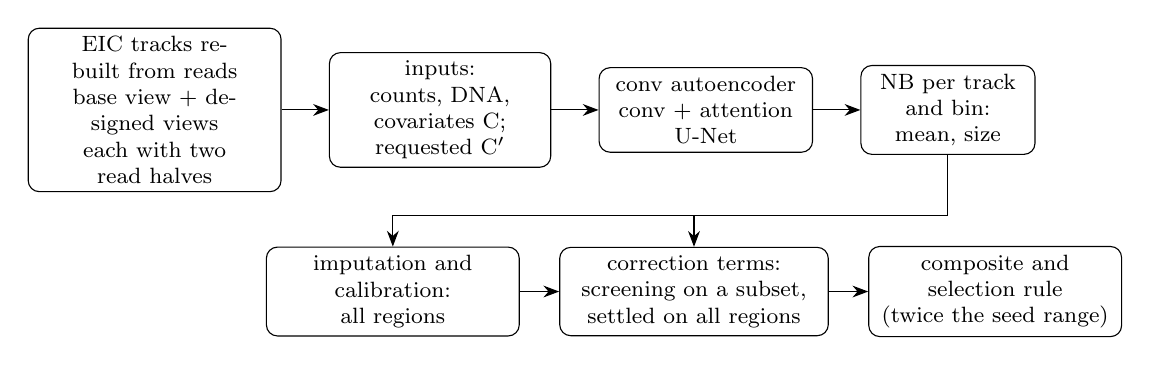
\begin{tikzpicture}[box/.style={draw, rounded corners, align=center, font=\footnotesize,
    minimum height=0.8cm, inner sep=3pt}, >={Stealth[length=2mm]}]
  \node[box, text width=3.0cm] (data) {EIC tracks rebuilt from reads\\ base view + designed views\\ each with two read halves};
  \node[box, text width=2.6cm, right=0.6cm of data] (in) {inputs: counts, DNA,\\ covariates C;\\ requested C$'$};
  \node[box, text width=2.5cm, right=0.6cm of in] (net) {conv autoencoder\\ conv + attention\\ U-Net};
  \node[box, text width=2.0cm, right=0.6cm of net] (nb) {NB per track\\ and bin:\\ mean, size};
  \draw[->] (data) -- (in);
  \draw[->] (in) -- (net);
  \draw[->] (net) -- (nb);
  \node[box, text width=3.0cm, below=1.0cm of in, xshift=-0.6cm] (imp) {imputation and\\ calibration:\\ all regions};
  \node[box, text width=3.2cm, right=0.5cm of imp] (cor) {correction terms:\\ screening on a subset,\\ settled on all regions};
  \node[box, text width=3.0cm, right=0.5cm of cor] (sel) {composite and\\ selection rule\\ (twice the seed range)};
  \draw[->] (nb.south) |- ($(imp.north)+(0,0.4)$) -- (imp.north);
  \draw[->] (nb.south) |- ($(cor.north)+(0,0.4)$) -- (cor.north);
  \draw[->] (imp.east) -- (cor.west);
  \draw[->] (cor) -- (sel);
\end{tikzpicture}
\caption{\cl{Design of the close-out. Every ablation changes one switch of a base recipe and trains with the same data, windows and seeds. All arms are scored on the same validation tracks. Imputation and calibration always use all regions; the correction terms use a subset of regions in the screening tier.}}\label{fig:design}
\end{figure}

\subsection{Metrics}

\cl{Each goal has one lead term on a scale where \lit{0} is a simple reference and \lit{1} is an ideal.}
\begin{itemize}
\item \cl{\textit{Imputation:} the share of the cell-type-specific variance recovered above the noise floor, $\lit{1} - (E - N)/(V - N)$, with $E$ the specific error, $V$ the specific variance of the truth and $N$ the pseudoreplicate noise floor. It is scored on \nItems{} validation items (\nItemsLoao{} with every other assay of the cell as input, \nItemsAcc{} with only an accessibility track as input).}
\item \cl{\textit{Correction:} the gap closed against depth-only scaling, $(c_{\text{depth}} - c_{\text{model}})/(c_{\text{depth}} - c_{\text{oracle}})$, where $c$ is the continuous ranked probability score (CRPS), i.e. the error of a full predictive distribution, and the oracle is the expected CRPS of the true sampling distribution of the target. It uses the \nCleanPairs{} never-trained crop pairs in \nCleanCells{} cells where neither side keeps duplicates; the other \nDupPairs{} pairs can share DNA fragments between source and target.}
\item \cl{\textit{Correction-only term:} the share of the covariate cost that the model closes, measured against its own same-view score. It is \lit{1} for a model that ignores its input, so it is read together with the correction term and is not in the composite.}
\item \cl{\textit{Calibration:} $\lit{1} - \text{PIT}_{\text{model}}/\text{PIT}_{\text{marginal}}$, where PIT is the mean gap between the probability integral transform curve and the diagonal, and the marginal is one constant NB per assay.}
\end{itemize}
\cl{The composite (version~\lit{3}) is $\lit{0.5}$ imputation $+ \lit{0.25}$ correction $+ \lit{0.25}$ calibration, each term clipped to $[\lit{0}, \lit{1}]$. This report quotes no raw CRPS value; every correction number is a ratio of CRPS differences, so the split of CRPS into its oracle-scaled and scale-error parts does not apply.}

\subsection{The selection rule and the seed range}

\cl{Each arm trains with \lit{3} seeds. The seed range is the maximum minus the minimum over the seeds. For an arm and its reference, the bar is the larger of the two seed ranges. An effect is ``beyond'' when the difference of means is larger than the bar; otherwise no claim is made. The selection rule, which was fixed before any run, adopts an arm only when its composite rises by more than twice the bar and no goal falls by more than twice its own bar; otherwise the simpler arm stays. With \lit{3} seeds the seed range is a rough estimate of the noise, and no correction for many comparisons is applied.}

\subsection{Region sampling and the two tiers}

\cl{The evaluation set has \nRegions{} regions of \nRegionBins{} bins, drawn at random from the genome mask. Imputation and calibration use all of them. A correction pair needs one prediction pass per region, so the screening tier scores pairs on \lit{16} evenly spaced regions. A check was written before any model score existed: \lit{16} regions become a settled tier only if six conditions hold on twelve runs (the three base recipes and the U-Net with DNA-only skip connections, \lit{3} seeds each). The conditions compare each subset value with a \lit{95}\% region-bootstrap interval of its \lit{256}-region value (\nBoot{} draws), the seed ranges, the selection-rule result and the rank order of the arms.}

\subsection{The ablations}

\cl{Sixteen ablations, i.e. groups of single-switch arms, ran on the conv autoencoder, conv + attention and the U-Net with \lit{3} seeds and \lit{80,000} windows each (\nArmRows{} arms, \nCells{} arm--model cells). They cover the ChIP control as input and output, an average-signal input, two-step routing through the base view, a fixed input depth, the DNA input and its fusion, the covariate embedding, injection and a scrambled-covariate control, the mask mode, four losses, the training views and nine count transforms. Each arm keeps the parameter budget within one percent of its base, except a few DNA-fusion and covariate-code arms.}

\section{Results and discussion}\label{sec:results}

\subsection{Three base models: a tie with a trade-off}

\cl{Table~\ref{tab:refs} gives the three base recipes. On the composite they are within the selection bar of each other. The U-Net recovers the most specific variance (\refUNImp{}, seed range \refUNImpR{}, against \refAEImp{} (\refAEImpR{}) for the conv autoencoder and \refATImp{} (\refATImpR{}) for conv + attention). The two convolutional models close the most correction gap (\refAECor{} (\refAECorR{}) and \refATCor{} (\refATCorR{}) against \refUNCor{} (\refUNCorR{})). All three are far above the position average (imputation \paImp{}, correction \paCor{}, calibration \paCal{}, composite \paComp{}). The axial transformer (composite \compAxial{}, range \compAxialR{}) and Perceiver IO (\compPerc{}, range \compPercR{}) were left out of the close-out by PI ruling.}

\cl{The trade-off survives on all \lit{256} regions (Table~\ref{tab:twofiftysix}): the U-Net closes less correction gap than the conv autoencoder by \dUnAeCorTwoFS{}, beyond its seed range, and the selection rule calls every one of the four comparisons a tie (U-Net below the conv autoencoder by \compAeUnAll{} against a bar of \compAeUnBar{}). A U-Net whose skip connections carry DNA features only moves to the profile of the convolutional models: correction \skipCor{} (\skipCorR{}) against \unCorTwoFS{}, and imputation \skipImp{} against \refUNImp{}. The count skips of the U-Net therefore buy imputation and cost correction. The tuned recipes of the last tuning round (composites \compTunAE{} (\compTunAER{}), \compTunAT{} (\compTunATR{}), \compTunUN{} (\compTunUNR{})) did not beat their bases beyond the seed range, and no architecture had converged at \lit{80,000} windows.}

\begin{table}[!htbp]
\caption{\cl{Base recipes on the screening tier. Mean (seed range) over \lit{3} seeds, \lit{80,000} windows. Imputation and calibration use all \lit{256} regions; correction, correction-only and the composite use \lit{16} pair regions.}}\label{tab:refs}
\footnotesize
\begin{tabular}{lccccc}
\toprule
model & imputation & correction & calibration & composite & correction-only \\
\midrule
\TabRefs
\botrule
\end{tabular}
\end{table}

\begin{table}[!htbp]
\caption{\cl{Correction terms on all \lit{256} regions for the four arms of the region check. Mean (seed range) over \lit{3} seeds.}}\label{tab:twofiftysix}
\footnotesize
\begin{tabular}{lcc}
\toprule
arm & correction (crop pairs) & correction-only \\
\midrule
\TabTwoFiftySix
\botrule
\end{tabular}
\end{table}

\subsection{The ablations}

\cl{Tables~\ref{tab:ablfull} and~\ref{tab:ablpairs} give every arm as arm minus base. Table~\ref{tab:ablfull} holds the two terms that are scored on all \lit{256} regions; Table~\ref{tab:ablpairs} holds the terms that rest on the \lit{16} pair regions and are screening results only. Over the \nCells{} arm--model cells, imputation fell beyond the bar in \nImpDn{} cells (\nImpDnTwo{} by more than twice the bar) and rose beyond it in \nImpUp{} (\nImpUpTwo{} by twice). The composite rose beyond the bar in \nCompUp{} cells and by twice the bar in \nCompUpTwo{}. Calibration moved beyond the bar in only \nCalDn{} cell, because its seed ranges are wide (\refUNCalR{} to \refAECalR{} for the bases).}

\cl{Four results are clear on the \lit{256}-region imputation term. First, the depth-removing count transforms hurt all three models by more than twice the bar: local ratio \eLrImpAE{}, \eLrImpAT{} and \eLrImpUN{}, per-window quantile \eQuImpAE{}, \eQuImpAT{} and \eQuImpUN{}. So the input must keep the depth scale. Second, covariates injected as tokens lowered U-Net imputation by \eTokImpUN{} (bar \eTokImpUNBar{}). Third, the ChIP control as an input and the DNA input help conv + attention only: removing the control gave \eCtlImpAT{} (bar \eCtlImpATBar{}), removing DNA \eDnaOffImpAT{} (bar \eDnaOffImpATBar{}), and DNA shifted by \lit{5}~Mb, a control for a misaligned sequence, \eShiftImpAT{} (bar \eShiftImpATBar{}). Fourth, the gains are single-model: the average-signal input raised U-Net imputation by \eAvgImpUN{} (bar \eAvgImpUNBar{}) and an imputation loss weight of \lit{4} raised conv + attention imputation by \eWfourImpAT{} (bar \eWfourImpATBar{}).}

\cl{Many arms are nulls on all three models: language-model DNA embeddings, adaLN-zero injection, covariate dropout, per-value numeric codes, the Poisson-mean loss and the drop mask mode moved no lead term beyond the bar. By the selection rule a null keeps the simpler or the incumbent value. The Anscombe transform is void: its output link has zero gradient at the zero-initialized head, so the mean never trained (imputation \anscImp{} on every seed). It is left out of the tables and needs a fix before a retrain.}

\cl{On the screening terms, the U-Net with a fixed input depth, i.e. every input thinned to \lit{$2^{23}$} reads, gained correction \eFixCorUN{} (bar \eFixCorUNBar{}) and composite \eFixCompUN{} (bar \eFixCompUNBar{}), but lost imputation \eFixImpUN{} (bar \eFixImpUNBar{}, a \lit{256}-region term). The PI noted that a fixed input depth can be unrealistic at deployment. Two-step routing through the base view at native depth lowered correction on both convolutional models (\eNatCorAE{}, bar \eNatCorAEBar{}; \eNatCorAT{}, bar \eNatCorATBar{}) and doubles the compute per window. Training with scrambled covariates lowered the correction-only term on all three models (\eScrCoAE{}, \eScrCoAT{}, \eScrCoUN{}; bars \eScrCoAEBar{}, \eScrCoATBar{}, \eScrCoUNBar{}), so the models use the covariates to correct a track. These effects rest on \lit{16} regions and are not settled (Section~\ref{sec:rescore}).}

\begin{table}[!htbp]
\caption{\cl{Ablations: terms scored on all \lit{256} regions. Arm minus base, per model (AE conv autoencoder, AT conv + attention, UN U-Net). $^{\dagger}$ beyond the bar (the larger seed range of arm and base); $^{\ddagger}$ beyond twice the bar; $^{a}$ two seeds; -- not run. Base values in Table~\ref{tab:refs}.}}\label{tab:ablfull}
\scriptsize
\begin{tabular}{lcccccc}
\toprule
 & \mcthree{imputation} & \mcthree{calibration} \\
arm & AE & AT & UN & AE & AT & UN \\
\midrule
\TabAblFull
\botrule
\end{tabular}
\end{table}

\begin{table}[!htbp]
\caption{\cl{Ablations: terms that use the \lit{16} pair regions (screening only). Arm minus base; marks as in Table~\ref{tab:ablfull}. The same-view-only U-Net arm has a raw correction value far below \lit{0} on two seeds, so its difference is not interpretable.}}\label{tab:ablpairs}
\tiny
\setlength{\tabcolsep}{2.6pt}
\begin{tabular}{lccccccccc}
\toprule
 & \mcthree{correction (crop pairs)} & \mcthree{correction-only} & \mcthree{composite} \\
arm & AE & AT & UN & AE & AT & UN & AE & AT & UN \\
\midrule
\TabAblPairs
\botrule
\end{tabular}
\end{table}

\subsection{Whether and where the counterfactual views help}

\cl{The PI asked whether the designed processing views help, and where. Fig.~\ref{fig:views} gives the answer per model. On the composite, training on the base view only is within the bar on all three models (\eBoCompAE{}, \eBoCompAT{}, \eBoCompUN{}; bars \eBoCompAEBar{}, \eBoCompATBar{}, \eBoCompUNBar{}). The composite cannot show a view effect, because its correction term uses only crop pairs, and no view arm moved them on the U-Net.}

\cl{The views help in three places. First, the correction-only term collapses without them on all three models: base view only gave \eBoCoAE{}, \eBoCoAT{} and \eBoCoUN{} (bars \eBoCoAEBar{}, \eBoCoATBar{}, \eBoCoUNBar{}), and adding the depth views alone did not restore it (\eBdCoAE{} on the conv autoencoder). Second, on the U-Net the depth-thinning views help on their own pairs: the two arms with depth views scored \thinWithLo{} to \thinWithHi{} on the thinning pairs in every seed, and every seed without them scored at most \thinWithoutHi{} (all views \thinAll{}, base only \thinBase{} with a very wide range). Third, models trained with all views keep imputation; the views do not cost imputation on any model.}

\cl{The views hurt in one place. Adding only the alignment-level views (no duplicate removal, no mapping-quality filter) lowered imputation on both convolutional models (\eBaImpAE{} and \eBaImpAT{}; bars \eBaImpAEBar{}, \eBaImpATBar{}) and correction (\eBaCorAE{}, \eBaCorAT{}). On the U-Net this arm scored \mnAlign{} (\mnAlignR{}) on the \nMnPairs{} pairs that mix the mapping-quality and duplicate knobs, against \mnAll{} for all views. A same-view-only arm raised imputation on the convolutional models (\eSvImpAE{}, \eSvImpAT{}) but broke the U-Net composite (\eSvCompUN{}, bar \eSvCompUNBar{}). The reading: the views are needed for the correction-only term and for depth correction, and the alignment-level views are harmful when trained without the others. The correction-only evidence is a \lit{16}-region screening result; it is one of the decisive arms of the rescoring.}

\begin{figure}[!htbp]
\centering
\begin{tikzpicture}
\begin{groupplot}[group style={group size=2 by 1, horizontal sep=0.6cm, yticklabels at=edge left},
    width=0.47\linewidth, height=5.0cm, ytick=data, y dir=reverse,
    yticklabels from table={\tblViewsCo}{label}, yticklabel style={font=\scriptsize},
    xticklabel style={font=\scriptsize}, xlabel style={font=\footnotesize},
    title style={font=\footnotesize}, enlarge y limits=0.12,
    extra x ticks={0}, extra x tick labels={}, extra x tick style={grid=major, grid style={gray}},
    unbounded coords=discard]
\nextgroupplot[title={(a) correction-only, \lit{16} regions}, xlabel={arm minus all views}]
  \addplot[only marks, mark=*, mark size=1.6pt, color=mAE, error bars/.cd, x dir=both, x explicit]
    table[x=dAE, y expr=\thisrow{y}-0.2, x error=bAE]{\tblViewsCo};
  \addplot[only marks, mark=square*, mark size=1.6pt, color=mAT, error bars/.cd, x dir=both, x explicit]
    table[x=dAT, y=y, x error=bAT]{\tblViewsCo};
  \addplot[only marks, mark=triangle*, mark size=2pt, color=mUN, error bars/.cd, x dir=both, x explicit]
    table[x=dUN, y expr=\thisrow{y}+0.2, x error=bUN]{\tblViewsCo};
\nextgroupplot[title={(b) imputation, \lit{256} regions}, xlabel={arm minus all views},
    legend style={font=\scriptsize, at={(-0.1,-0.40)}, anchor=north, legend columns=3}]
  \addplot[only marks, mark=*, mark size=1.6pt, color=mAE, error bars/.cd, x dir=both, x explicit]
    table[x=dAE, y expr=\thisrow{y}-0.2, x error=bAE]{\tblViewsImp};
  \addplot[only marks, mark=square*, mark size=1.6pt, color=mAT, error bars/.cd, x dir=both, x explicit]
    table[x=dAT, y=y, x error=bAT]{\tblViewsImp};
  \addplot[only marks, mark=triangle*, mark size=2pt, color=mUN, error bars/.cd, x dir=both, x explicit]
    table[x=dUN, y expr=\thisrow{y}+0.2, x error=bUN]{\tblViewsImp};
  \legend{conv autoencoder, conv + attention, U-Net}
\end{groupplot}
\end{tikzpicture}
\caption{\cl{Training views against the all-views reference. Each point is arm minus reference; the error bar is $\pm$ the bar (the larger seed range of arm and reference), so a bar that does not cross \lit{0} is an effect beyond the seed range. (a) The correction-only term falls on all three models without the processing views. (b) Imputation falls only with the alignment-level views on the convolutional models. The U-Net same-view-only correction-only value is undefined and is not drawn.}}\label{fig:views}
\end{figure}

\subsection{The check of \lit{16} against \lit{256} pair regions failed}

\cl{The check ran on twelve runs with \nBoot{} region-bootstrap draws over \nClusters{} clusters. No size of \lit{8}, \lit{16} or \lit{32} regions passed all six conditions (Table~\ref{tab:check}). At \lit{16} regions, \condOneP{} of \condOneN{} subset values fell inside the \lit{95}\% interval of their \lit{256}-region value (condition~\lit{1}), only \condTwoShare{}\% of the per-assay cells did (condition~\lit{2}), \condFourP{} of \condFourN{} seed ranges stayed within \lit{1.5} times their \lit{256}-region value (condition~\lit{4}), and \condSixP{} of \condSixN{} rank orders kept their sign (condition~\lit{6}). The selection-rule result held for all four comparisons (condition~\lit{3}).}

\cl{Fig.~\ref{fig:region} shows the failure per run and seed. For the crop-pair correction term \inCorP{} of \inCorN{} run-seeds were inside the interval, but for the correction-only term only \inCoP{} of \inCoN{} were: on the two convolutional models the \lit{16}-region value was higher than the \lit{256}-region interval on every seed. So the pre-written rule applies: correction terms are scored on all \lit{256} regions from now on, and every \lit{16}-region correction effect in this report is a screening result.}

\cl{The \lit{16} regions are not ``dead'' regions. Their median signal is at the \pairPct{}th percentile of all \nCandBlocks{} candidate blocks, and the poorest is at the \pairLowPct{}th. A bootstrap of the \lit{16} regions found that every ablation effect beyond the seed range kept its sign in at least \lit{95}\% of \nResample{} resamples. One region carries much weight: without it the U-Net correction-only effect of the quantile transform falls from \regNinetySix{} to \regNinetySixTo{}. The two checks answer different questions. The bootstrap says the effects hold for regions like the \lit{16}; the failed check says the \lit{16} do not reproduce the \lit{256}-region values.}

\begin{table}[!htbp]
\caption{\cl{The pre-written check of the pair regions: pass or fail per condition and size. A size passes only when all six conditions pass.}}\label{tab:check}
\footnotesize
\setlength{\tabcolsep}{3pt}
\begin{tabular}{lccccccc}
\toprule
regions & (\lit{1}) interval & (\lit{2}) per assay & (\lit{3}) rule result & (\lit{4}) seed range & (\lit{5}) variance ratio & (\lit{6}) rank & all \\
\midrule
\TabCheck
\botrule
\end{tabular}
\end{table}

\begin{figure}[!htbp]
\centering
\begin{tikzpicture}
\begin{groupplot}[group style={group size=2 by 1, horizontal sep=0.6cm, yticklabels at=edge left},
    width=0.47\linewidth, height=5.6cm, ytick=data, y dir=reverse,
    yticklabels from table={\tblRegion}{label}, yticklabel style={font=\tiny},
    xticklabel style={font=\scriptsize}, xlabel style={font=\footnotesize},
    title style={font=\footnotesize}, enlarge y limits=0.04]
\nextgroupplot[title={(a) correction, crop pairs}, xlabel={term value}]
  \addplot[only marks, mark=none, color=mgray, error bars/.cd, x dir=both, x explicit]
    table[x=ca, y=y, x error plus expr=\thisrow{chi}-\thisrow{ca}, x error minus expr=\thisrow{ca}-\thisrow{clo}]{\tblRegion};
  \addplot[only marks, mark=*, mark size=1.4pt, color=mUN] table[x=cs, y=y]{\tblRegion};
\nextgroupplot[title={(b) correction-only}, xlabel={term value}]
  \addplot[only marks, mark=none, color=mgray, error bars/.cd, x dir=both, x explicit]
    table[x=oa, y=y, x error plus expr=\thisrow{ohi}-\thisrow{oa}, x error minus expr=\thisrow{oa}-\thisrow{olo}]{\tblRegion};
  \addplot[only marks, mark=*, mark size=1.4pt, color=mUN] table[x=os, y=y]{\tblRegion};
\end{groupplot}
\end{tikzpicture}
\caption{\cl{Value on \lit{16} pair regions (red dot) against the \lit{256}-region value (gray dot) and its \lit{95}\% region-bootstrap interval (gray bar), per run and seed. A dot outside its bar fails condition~\lit{1}. (a) The crop-pair correction term is mostly inside. (b) The correction-only term of the convolutional models is above the interval on every seed.}}\label{fig:region}
\end{figure}

\subsection{The \lit{256}-region rescoring of the decisive arms}\label{sec:rescore}

%% RESCORING-PARAGRAPH START (replace this paragraph when the 256-region scores land)
\cl{\textbf{[Waits for the rescoring.]} Seven decisive arms (\lit{21} arm folders, \rescoreSeeds{} run-seeds) must be scored on all \lit{256} regions before any correction effect of the ablations can settle: the scrambled covariates, base view only, two-step at native and at fixed base depth, fixed input depth, the average-signal input, and imputation weight \lit{4}. The cost is \rescoreCost{} allocated CPU-hours (\nRunsAE{} conv autoencoder run-seeds at \costAE{}, \nRunsAT{} conv + attention at \costAT{}, \nRunsUN{} U-Net at about \costUN{} each). \textit{Status:} by PI decision the scoring runs on Nibi, since \rsDay{}, \rsStart{} UTC (run log): \rsN{} run-seeds, \rsCap{} at one time, about \rsHours{}~h per scoring, and \rsScored{} of \rsN{} scored at \rsNow{} UTC on \rsNowDay{}. At this rate the predict stage needs \rsRounds{} rounds, about \rsTotal{}~h, so most scores land after the run ends. Table~\ref{tab:rescore} gives the \lit{16}-region effects and leaves the \lit{256}-region columns empty. The settled-design document states, before any result, the rule that each arm's \lit{256}-region effect will apply.}
%% RESCORING-PARAGRAPH END

%% RESCORING-TABLE START (the 256-region columns fill themselves from the build hook)
\begin{table}[!htbp]
\caption{\cl{The seven decisive arms: effects on the two correction terms, arm minus base. The \lit{16}-region columns are screening results; the \lit{256}-region columns wait for the rescoring. Marks as in Table~\ref{tab:ablfull}.}}\label{tab:rescore}
\scriptsize
\begin{tabular}{llcccc}
\toprule
 & & \mctwo{\lit{16} regions} & \mctwo{\lit{256} regions} \\
arm & model & correction & correction-only & correction & correction-only \\
\midrule
\TabRescore
\botrule
\end{tabular}
\end{table}
%% RESCORING-TABLE END

\subsection{Signal p-value and peaks from the predicted distribution}

\cl{The EIC scores a signal track, i.e. the $-\log_{\lit{10}}$ p-value of the \lit{MACS2} peak caller, not counts. We derive this track from the predicted NB after training. The first formula used the count in each bin alone (the in-bin pileup). It has a known flaw: it does not spread a read to the bins that its fragment covers, so the pileup is too spiky, it overstates the counting noise of a pileup built from a predicted NB, and it over-calls peaks. On the observed counts of \nFormTargets{} validation targets (\nFormChip{} ChIP-seq) we tested \nVariants{} pileup variants against the pipeline's own track (Table~\ref{tab:formula}). The box-spread variant, i.e. each count spread over a centred box of the fragment length, raised the agreement and the peak precision, and the PI adopted it. It is a fitted choice among \nVariants{} variants, not a derivation; the strand and the base-pair position are lost at binning, so no formula on \lit{25}~bp counts can reproduce the pipeline exactly.}

\cl{Only one run-seed has a signal-space score, and it used the flawed in-bin formula: the conv autoencoder, seed \lit{0}, recovered \eTwoSigExp{} of the specific variance in signal space against \eTwoCounts{} in counts (mean over \eTwoNAssays{} assays), and \eTwoSigPc{} when the control was also predicted. These values carry the flaw and have no seed range. The predicted control was close to the observed one: the median ratio was \lamVisible{} when the control was an input (\lamVisibleK{} of \lamVisibleN{} targets within \lit{10}\%) and \lamHidden{} when it was hidden (\lamHiddenK{} of \lamHiddenN{}). The rescoring of the base runs with the box spread is queued.}

\begin{table}[!htbp]
\caption{\cl{Signal formula on observed counts against the pipeline track: median over targets. Peaks are \lit{500}~bp tiles at $-\log_{\lit{10}} p \ge \lit{2}$.}}\label{tab:formula}
\footnotesize
\begin{tabular}{lcc}
\toprule
measure & in-bin pileup (superseded) & box spread (adopted) \\
\midrule
\TabFormula
\botrule
\end{tabular}
\end{table}

\subsection{Second experiments, lab and donor}

\cl{A second experiment is another ENCODE experiment of the same cell and assay. The add-on tables append \nSecond{} such rows (\nSecondOther{} from another lab, \nSecondSame{} from the same lab), with \nSecondVal{} validation targets; the leak checks passed with every count at zero. The PI decided two points on \lit{2026-11-17}. First, lab is reported together with donor as one effect, because a pair with another lab and the same donor comes from only two cells in every assay class. Second, the \dTwoDropped{} unbuilt DNase-seq second-experiment rows are dropped, so the add-on stays at \dTwoKept{} experiments.}

\cl{The variance layers of these pairs ran on the real data (pair value as in the ladder; rows pooled by assay class; \lit{95}\% cluster-bootstrap intervals). Over the biological replicate, all second-experiment pairs of broad histone marks gave \dTwoBrAll{} [\dTwoBrAllLo{}, \dTwoBrAllHi{}] (\dTwoBrAllN{} pairs, \dTwoBrAllC{} cells), and lab with donor gave \dTwoBrLd{} [\dTwoBrLdLo{}, \dTwoBrLdHi{}] (\dTwoBrLdN{} pairs, \dTwoBrLdC{} cells). For narrow histone marks the values were \dTwoNrAll{} [\dTwoNrAllLo{}, \dTwoNrAllHi{}] (\dTwoNrAllN{} pairs, \dTwoNrAllC{} cells) and \dTwoNrLd{} [\dTwoNrLdLo{}, \dTwoNrLdHi{}] (\dTwoNrLdN{} pairs, \dTwoNrLdC{} cells). Every interval includes zero, so these pairs resolve no variance of lab with donor beyond a biological replicate. In \dTwoBrLdTech{} of the \dTwoBrLdN{} broad lab-with-donor pairs the two sides also differ in run type, read length or platform. The accessibility classes have at most \dTwoSmall{} pairs. These pooled rows use other cells than the rung below, so the assay-matched ladder below is the primary value. No model ran on these pairs.}

\subsection{The replicate ladder}

\cl{The replicate ladder splits the pair value $\lit{0.5}\,E[(Y-Y')^{\lit{2}}]$ of two tracks, i.e. the expected squared difference of their log counts at a common depth, into nested layers. Each rung adds one difference to the rung below it: read sampling (two read halves of one library), a biological replicate, a second experiment, and another cell type. The increment of a rung is assay-matched: on each cell and assay with pairs of both rungs, the pair value of the rung minus that of the rung below, then a mean over assays and cells. A rung is estimable with at least \minPairs{} matched pairs from \lit{3} cells. By PI decision of \lit{2026-11-17} the ladder subtracts two-sided, with the check on common cell types, so earlier ladder numbers (the one-sided smoke run on \lit{H3K36me3}) are not comparable. On the units that hold the sampling, replicate and cell-type rungs, the three increments add up exactly to the cell-type pair value in \ladChainOk{} of \ladChainN{} groups.}

\cl{Table~\ref{tab:ladder} gives every estimable rung. Read sampling holds most of the cell-type pair value: \ladBrSamp{} in broad marks, \ladNrSamp{} in narrow marks, and \ladDnSamp{} in DNase-seq, where the cell-type pair value is at the level of read sampling. The biological replicate adds \ladBrRep{} and \ladNrRep{}, and in DNase-seq its increment is negative (\ladDnRepInc{}, share \ladDnRep{}); its interval includes zero. The cell type adds \ladBrCt{}, \ladNrCt{} and \ladDnCt{}. Above the replicate only two rows are estimable: lab with donor in broad marks, which is negative (\ladBrLd{}, \ladBrLdSh{}), and an experiment repeat with another donor in narrow marks; both intervals include zero. Negative increments are kept, not clipped. ATAC-seq has no estimable rung (\ladAtacN{} read-half pairs from \ladAtacC{} cells). Three kinds of rung are not estimable. First, the sequencing and library rungs are empty, because the per-library and per-lane units were never built. Second, no pair in the challenge data holds two donors inside one experiment. Third, the other second-experiment rows have too few matched pairs or cells, for example lab alone in broad marks (\ladBrLabN{} pairs from \ladBrLabC{} cells). The crossed mixed model did not run: it needs a noise level per library first.}

\begin{table}[!htbp]
\caption{\cl{The replicate ladder, two-sided and assay-matched, all regions and signal bands. Increment over the rung below (pair value of log counts) with its \lit{95}\% cluster-bootstrap interval; share of the cell-type pair value on the same cells and assays (number of those units).}}\label{tab:ladder}
\scriptsize
\setlength{\tabcolsep}{3.5pt}
\begin{tabular}{llccc}
\toprule
assay class & rung & pairs (cells) & increment [\lit{95}\% interval] & share (units) \\
\midrule
\TabLadder
\botrule
\end{tabular}
\end{table}

\subsection{The settled design}

\cl{Table~\ref{tab:design} condenses the settled-design document. ``Settled'' means that no planned run can change the value or that the PI fixed it; ``provisional'' means that a named run can change it. The design tests gave \testsPassed{} passed, \testsSkipped{} skipped and \testsFailed{} failed. The failure was a configuration-key guard that would stop every run of the covariate-set search; a later commit on the run branch fixed it.}

\cl{Every model beats the position average by more than twice its seed range on imputation and calibration. On the \lit{16}-region correction term both convolutional models do too, and the U-Net does not: its margin is \dTwoMarginUN{} against twice its seed range, \dTwoBarUN{}.}

\begin{table}[!htbp]
\caption{\cl{The settled miniCANDI design, condensed. Confidence and status are the agent's reading of the evidence, written before the rescoring.}}\label{tab:design}
\scriptsize
\begin{tabular}{p{2.8cm}p{4.3cm}p{2.0cm}p{2.9cm}}
\toprule
choice & value & confidence & status \\
\midrule
architecture & conv autoencoder, conv + attention and U-Net carried forward; tie with a trade-off & moderate & settled tie; the pick is the PI's \\
count input & offset, $\log_{\lit{2}}((y+\lit{1})/s)$ & strong against local ratio and quantile & settled \\
covariate injection & FiLM & moderate & settled; concatenation open on conv + attention \\
covariate set & \lit{11} metadata columns, no QC columns & weak & value by PI ruling; field set provisional \\
mask mode & learned token (drop is equal) & moderate null & settled \\
ChIP control & input and output & weak; output by ruling & settled \\
DNA & own tower, early join & weak & settled \\
loss & NB negative log-likelihood, weights \lit{1}/\lit{1}/\lit{1} & moderate against Poisson & provisional (weight \lit{4}, NB CRPS) \\
training views & all views & weak (\lit{16}-region term) & provisional (rescoring) \\
two-step routing & off & moderate & provisional (rescoring) \\
input depth & native & weak & provisional (rescoring, mix round) \\
average-signal input & off & weak & provisional (U-Net) \\
resolution, context & \lit{25}~bp, \lit{1,024} bins & by ruling & settled for this run \\
training length & \lit{80,000} windows & weak (no model converged) & provisional \\
QC on input, cell embedding & off, none & not tested & provisional \\
\botrule
\end{tabular}
\end{table}

\subsection{Discussion}

\cl{The data and the evaluation are the solid part of the close-out. The rebuilt tables separate processing variance from biology by design, every view has read halves, and the scorer passed exact validity checks on its references. The design part is weaker. Most effects that are large enough to show beyond the seed range are on the imputation term or on correction terms that rest on \lit{16} regions, and most single gains hold on one model only. With \lit{3} seeds, ranges as wide as \refAECalR{} on calibration hide effects of that size, and the many comparisons of the tables make a few false ``beyond'' marks likely.}

\cl{Three readings carry over to scaling with moderate confidence. First, the input must keep the depth scale: every depth-removing transform hurt imputation on all three models, and an earlier arm that hid the depth covariate cut the U-Net composite. Second, the architecture choice is a choice between goals: the count skips of the U-Net raise imputation and lower correction. Third, the counterfactual views are needed for the correction-only term and for depth correction, and they cost no imputation when all views train together. The third reading rests on \lit{16}-region scores until the rescoring runs.}

\cl{Several numbers told to the PI during the run were later corrected. The cost of one \lit{256}-region scoring was first quoted as \oldScoreCost{} CPU-hours; the measured cost is \costAE{} to about \costUN{}. The cost of the rescoring rose from \oldCheckCost{} to \rescoreCost{} CPU-hours, the blind build from \blindOldCost{} CPU-hours used to about \blindNewCost{} allocated, and the mix-and-match round fell from \mixOldCost{} to \mixCost{}. The composite changed definition twice; every composite in this report is version~\lit{3}.}

\subsection{Data deliverables of the last night}

\cl{The QC side tables hold read-derived quality metrics per row. The fill wrote \qcWhole{} records for the base pass and \qcPrOne{} for the read halves (\qcOk{} ok, \qcNoRead{} without a read set, \qcRefused{} refused). Over the \qcRows{} training and validation rows, NSC and RSC are filled for \qcNsc{} (\qcNscPct{}\%), the fragment length for \qcFrag{} (\qcFragPct{}\%), and NRF, \lit{PBC1} and \lit{PBC2} for \qcNrf{} (\qcNrfPct{}\%), because they exist only for the base and no-duplicate-removal views. FRiP is filled for \qcFrip{} rows, because this pass calls no peaks. The \lit{1}~bp region store holds \bpViews{} recounted views; an independent count matched \bpPts{} of \bpPtsStore{} points, and the table build, which refuses a view without a passed read-set check, wrote \bpMeas{} measurements and \bpPairs{} pairs. Its verification and the variance by bin size still run. Before any removal, four scratch folders went to tape as \arcTars{} tar files (\arcGib{} GiB), each compared with scratch. The removals took Nibi scratch from \scBefore{} to \scMid{} and then to \scAfter{} GiB, under the soft quota, and writes resumed.}

\subsection{What did not run, and why}

\cl{Three limits stopped work in the last two days. First, Fir entered a planned outage on \lit{2026-11-17} that lasts to about \lit{2026-11-20}; \firQueued{} jobs wait in its queue, among them the twelve matched-compute trainings and the Fir copies of the rescoring. Second, Nibi scratch refused every write until the last night: use was \nibiUsed{} GiB against a soft quota of \nibiQuota{} GiB, and the work folder of \nibiWork{} GiB could leave only after the QC fill and the recount that read it. Third, the PI gave the run \lit{24} hours to close, so no new training round started. The run used \tallyTotal{} allocated CPU-hours from \lit{2026-11-10} to \lit{2026-11-17} (Fir \tallyFir{}, Nibi \tallyNibi{}). Not run: the mix-and-match round, the minimum covariate set, the learned cell-type embedding, QC metrics on the input, RNA-seq input, the resolution arms, the pointwise model under the corrected composite, the blind build and the final model.}

\begin{table}[!htbp]
\caption{\cl{The ready queue for the next session, from the ready-queue document. Cost in allocated CPU-hours.}}\label{tab:queue}
\tiny
\begin{tabular}{rp{6.2cm}p{2.6cm}p{3.6cm}}
\toprule
order & entry & cluster & CPU-hours \\
\midrule
\TabQueue
\botrule
\end{tabular}
\end{table}

\subsection{Decisions taken and decisions moved}

\cl{On \lit{2026-11-17} the PI took \nDecisions{} decisions, one at a time (Table~\ref{tab:decisions}). Decisions \lit{1} to \lit{5} act in this window; decisions \lit{6} to \lit{9} fix the scope and budget of runs in the next session. The PI moved two decisions to the next session: the architecture that goes to scaling, and the data version of the final model. The PI's words: ``\piQuoteScale{}''; on the data version, ``\piQuoteData{}''. The settled-design document informs both and recommends, as the agent's intent, carrying the conv autoencoder and the U-Net into the first scaling step, with the choice after the mix-and-match round, and building the table version that makes DNase-seq scorable for correction before the final model trains.}

\begin{table}[!htbp]
\caption{\cl{The PI decisions of \lit{2026-11-17}, from the decision record. Costs are allocated CPU-hours.}}\label{tab:decisions}
\tiny
\setlength{\tabcolsep}{3pt}
\begin{tabular}{rp{3.6cm}p{4.4cm}p{5.6cm}}
\toprule
 & decision & PI choice & consequence \\
\midrule
\TabDecisions
\botrule
\end{tabular}
\end{table}

\section{Conclusion}\label{sec:conclusion}

\cl{The data criterion is partial: the tables, views, halves, covariates and second experiments exist, and the blind build does not. The objective criterion is delivered. The evaluation criterion is partial: the metrics and the scorer are defined and tested, and the replicate ladder shows that read sampling holds most of the cell-type pair value; but the screening tier failed its check, so the correction terms need \lit{256} regions, and that rescoring has not landed. The design criterion is partial: three architectures tie with a trade-off between imputation and correction, the count input with a depth offset is settled, and the rows on views, two-step routing, input depth and loss weights stay provisional.}

\cl{The main limitations are the \lit{16}-region correction terms, \lit{3} seeds per arm, models that had not converged at \lit{80,000} windows, and ablations on the first table version.}

\cl{The next session starts from the ready queue (Table~\ref{tab:queue}): the rescoring settles every correction effect, the mix-and-match round (\mixCost{} CPU-hours plus a gate of \mixGate{}) tests whether gains combine, and the final model gives the EIC board row.}


\end{document}
